\documentclass[a4paper,10pt,openright]{report}
\setlength{\parindent}{0pt} % set noindent for entire file

\usepackage[utf8]{inputenc}
\usepackage[a4paper, top=2cm, left=1cm, right=1.5cm]{geometry}
\usepackage{xcolor,graphicx}
\usepackage{amsmath}
\usepackage{setspace}
\usepackage{sectsty}
\usepackage{etoolbox}
\usepackage{enumitem}
\usepackage{listings}
\usepackage{times}

\graphicspath{ {/home/saran/Analytics/May_05/} }

\lstdefinestyle{mystyle}{
	backgroundcolor=\color{white},
	basicstyle=\ttfamily\footnotesize,
	breakatwhitespace=false,
	breaklines=true,
	captionpos=b,
	keepspaces=true,
	showspaces=false,
	showstringspaces=false,
	showtabs=false,
	tabsize=4
}

\lstset{style=mystyle}

\begin{document}
\singlespacing
\pagestyle{plain}

\begin{center}
\textbf{Assignment Z-test} \\
Date: 05/05/2020 \hspace{2mm} Name: D.Saravanan
\end{center}

\vspace{10px}

TTest test the null hypothesis $H_{0}$ against the alternative hypothesis $H_{1}$. \\

For univariate samples, TTest performs a Student $t$ test. The test statistic is assumed to
follow a StudentTDistribution [df]. \\ 

The degrees of freedom df, used to specify the distribution of the test statistic, depend on
the sample size, number of samples, and in the case of two univariate samples, the results 
of a test for equal variances. \\ 

For the TTest, a cutoff $\alpha$ is chosen such that $H_{0}$ is rejected only if $p < \alpha
$. The value of $\alpha$ used for the "TestConclusion" and "ShortTestConclusion" properties 
is controlled by the SignificanceLevel option. This value $\alpha$ is also used in diagnostic
tests of assumptions, including tests for normality, equal variance, and symmetry. By 
default, $\alpha$ is set to $0.05$. 

\begin{enumerate}

\item[1.] A sample of 400 male students is found to have a mean height of 171.38 cm. Can it
be reasonably regarded as a sample from a large population with mean height 171.17 cm and
standard deviation 3.30 cm.

Null hypothesis: $H_{0}: \mu = 16$ \\
Alternative hypothesis: $H_{1}: \mu \neq 16$ 

\begin{enumerate}
\item[(i)] $\bar x = 16.35$, $s = 0.5$ and $n = 25$ 

\begin{equation*}
t = \frac{\bar x - \mu}{s/\sqrt{n}}
  = \frac{16.35 - 16}{0.5/\sqrt{25}} 
  = 3.5
\end{equation*}

\item[(ii)] $\bar x = 15.8$, $s = 0.5$ and $n = 25$

\begin{equation*}
t = \frac{\bar x - \mu}{s/\sqrt{n}}
  = \frac{15.8 - 16}{0.5/\sqrt{25}}
  = -2.0
\end{equation*}	

\vspace{0.5cm}

Program:
\lstinputlisting[language=Python]{tscript.py}

Output:
\lstinputlisting{toutput1a.txt}

%figure_1
\begin{figure}[ht!]
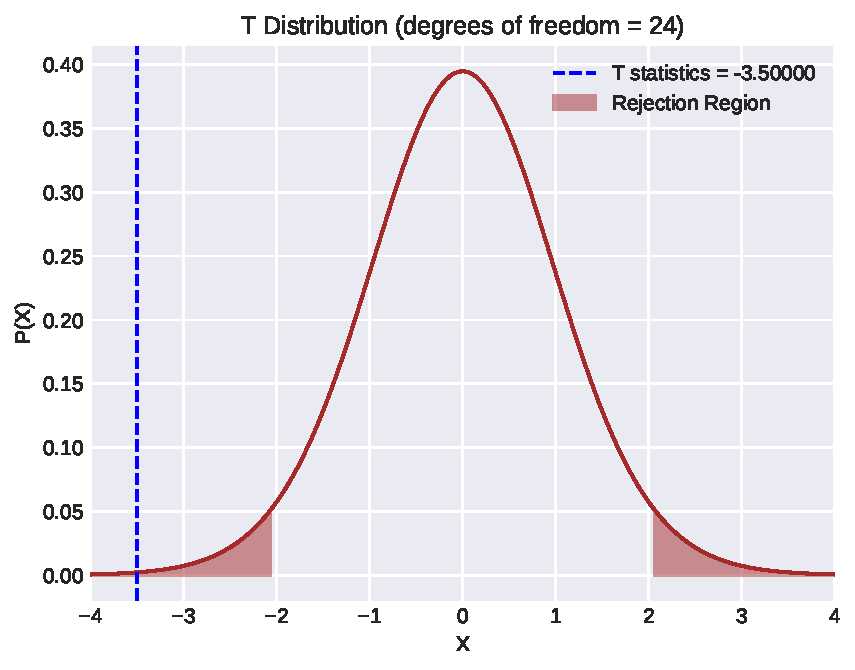
\includegraphics[width=14cm,height=7cm,keepaspectratio]{tscript1a.pdf}
\centering
\end{figure}

\pagebreak

\lstinputlisting{toutput1b.txt}

%figure_2
\begin{figure}[ht!]
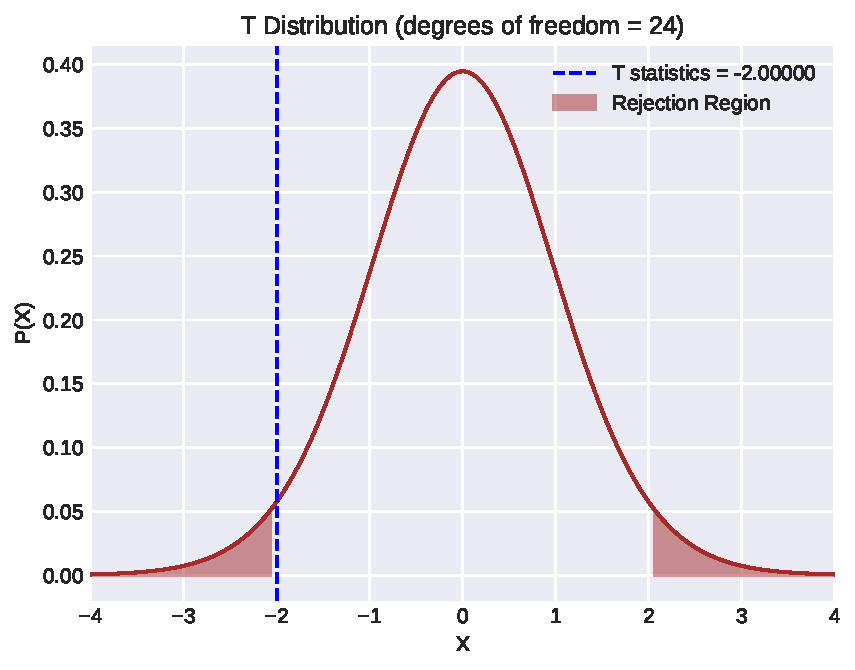
\includegraphics[width=14cm,height=7cm,keepaspectratio]{tscript1b.pdf}
\centering
\end{figure}

\end{enumerate}

\item[2.] A sample of 900 items has mean 3.4 and standard deviation 2.61 Can the sample be
regarded as drawn from a population with mean 3.25 at 1 percent level of significane. \\

Null hypothesis: $H_{0}: \mu = 5$ \\
Alternative hypothesis: $H_{1}: \mu \neq 5$ \\

Sample mean:
\begin{equation*}
\bar x =  \frac{\sum\limits_{i=1}^{n} x_{i}}{n} 
	= \frac{4.7 + 4.9 + 5.0 + 5.1 + 5.4 + 5.2 + 4.6 + 5.1 + 4.6 + 4.7}{10} 
	= 4.93
\end{equation*}

Sample variance:
\begin{equation*}
s^{2} = \frac{\sum\limits_{i=1}^{n} (x_{i} - \bar x)^{2}}{n - 1} 
	= \frac{\sum\limits_{i=1}^{10} (x_{i} - 4.93)^{2}}{10-1} 
	= 0.0681
\end{equation*}

Sample standard deviation:
\begin{equation*}
s = \sqrt{\frac{\sum\limits_{i=1}^{n} (x_{i} - \bar x)^{2}}{n - 1}}
= \sqrt{\frac{\sum\limits_{i=1}^{10} (x_{i} - 4.93)^{2}}{10 - 1}}
= \sqrt{0.0681} = 0.26096
\end{equation*}

T-statistics:
\begin{equation*}
t = \frac{\bar x - \mu}{s/\sqrt{n}} = \frac{4.93 - 5}{0.26096/\sqrt{10}} = -0.84825
\end{equation*}

\vspace{1.5cm}

Program:
\lstinputlisting[language=Python]{tscript2.py}

\pagebreak

Output:
\lstinputlisting{toutput2.txt}

%figure_3
\begin{figure}[ht!]
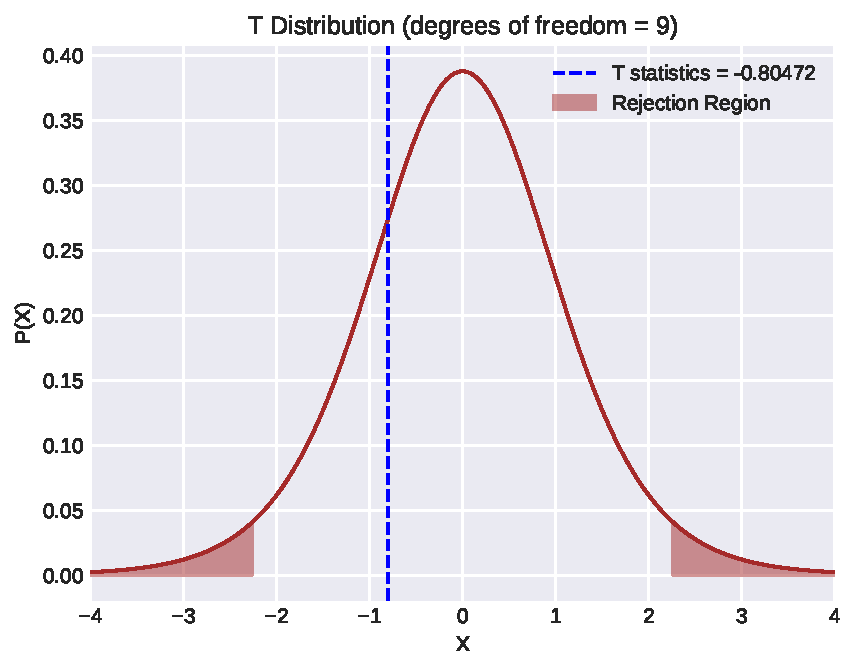
\includegraphics[width=14cm,height=7cm,keepaspectratio]{tscript2.pdf}
\centering
\end{figure}

\item[3.] Two sets of ten students selected at random from a college were taken. One set was
given memory test as they were and the other was given the memory test after two weeks of
training and the scores are given below. \\
\begin{tabular}{lrrrrrrrrrr}
Set A: & 10 & 8 & 7 & 9 & 8 & 10 & 9 & 6 & 7 & 8 \\
Set B: & 12 & 8 & 8 & 10 & 8 & 11 & 9 & 8 & 9 & 9 \\
\end{tabular} \\
Do you think there is a significant effect due to training? \\

Program:
\lstinputlisting[language=Python]{tscript3.py}
Output:
%\lstinputlisting{tscript3.txt}

\end{enumerate}
\end{document}
